\chapter{Аналитический раздел}

В данном разделе рассмотрены основные понятия рассматриваемой предметной области, а также проведен обзор существующих методов повышения разрешения изображения по нескольким кадрам.

\section{Общие термины и понятия предметной области}

Изображение, получаемое цифровой фотокамерой, можно определить как двумерную функцию $f(x,\;y)$, где $x$ и $y$ --- пространственные координаты, принимающие конечное число дискретных значений. Значение функции $f$ в некоторой точке, задаваемой парой координат $(x, y)$, является положительной скалярной величиной, называемой интенсивностью, или яркостью (уровнем серого) изображения в этой точке~\cite{digital_pic_1, digital_pic_2}. 

В контексте данной работы под термином <<кадр>> понимается предоставляемое цифровое изображение низкого разрешения, используемое для синтеза изображения высокого разрешения. Каждый кадр является изображением одного и того же объекта, незначительно смещенного относительно других кадров из набора.

Чем больше количество точек (пикселей) на единицу площади изображения, тем выше его разрешение. Такие изображения предоставляют больше информации о деталях, учет которых может быть критически важен для различного рода задач (таких как медицина, наблюдения за спутниками, видеонаблюдение).

На рисунке \ref{model} представлена модель наблюдения изображения низкого разрешения.

\begin{figure}[H]
	\centering
	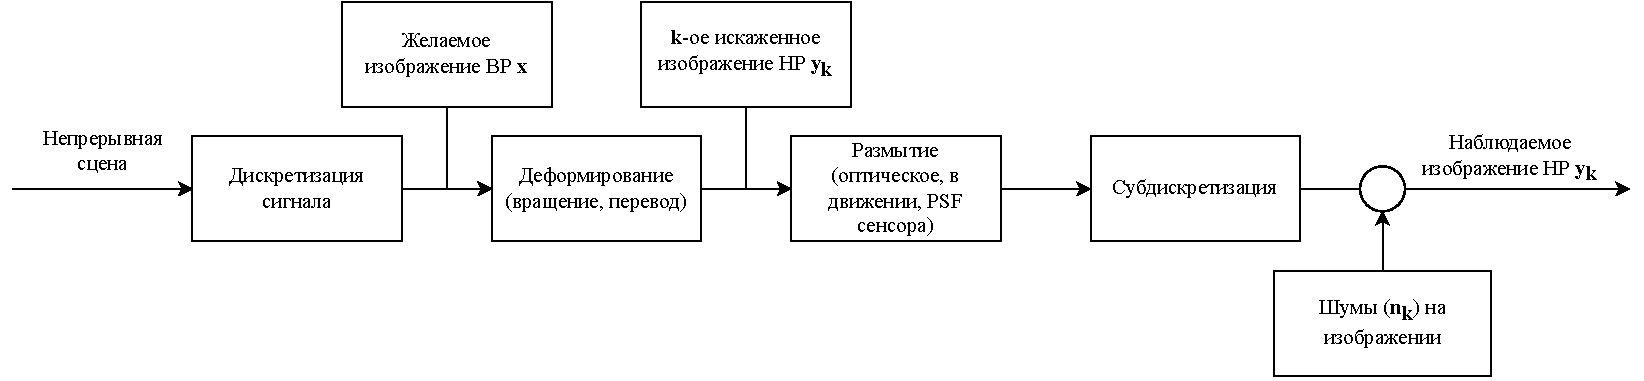
\includegraphics[scale=0.6]{assets/model}
	\caption{Модель наблюдения изображения низкого разрешения}
	\label{model}
\end{figure}

Задача повышения разрешения изображения по одному или нескольким кадрам низкого разрешения получила название суперразрешения (англ.~\textit{super~resolution})~\cite{n1, n2, n3}. В общем случае эта задача является некорректной, т.к. в реальных задачах сведения об искажениях изображения заведомо неизвестны.

На рисунке \ref{shoots} представлен пример фиксации положений движущегося объекта.
 
\begin{figure}[h!]
    \centering
    \begin{subfigure}{0.17\textwidth}
        \centering
        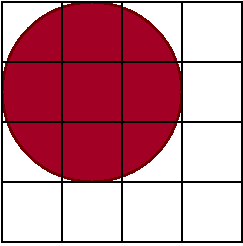
\includegraphics[width=\textwidth]{assets/c1.pdf}
        \caption{Положение №1}
    \end{subfigure}
    \begin{subfigure}{0.17\textwidth}
        \centering
        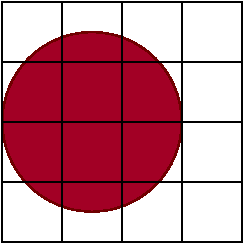
\includegraphics[width=\textwidth]{assets/c2.pdf}
        \caption{Положение №2}
    \end{subfigure}
    \begin{subfigure}{0.17\textwidth}
        \centering
        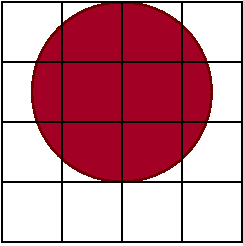
\includegraphics[width=\textwidth]{assets/c3.pdf}
        \caption{Положение №3}
    \end{subfigure}
    \begin{subfigure}{0.17\textwidth}
        \centering
        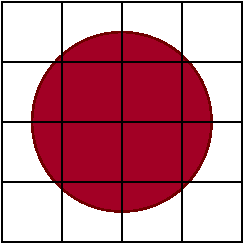
\includegraphics[width=\textwidth]{assets/c4.pdf}
        \caption{Положение №4}
    \end{subfigure}
    \caption{Пример фиксации положений движущегося объекта}
    \label{shoots}
\end{figure}

На рисунке \ref{circles} представлен пример набора кадров одного и того же объекта, регистрируемого фотосистемой.

\begin{figure}[h!]
    \centering
    \begin{subfigure}{0.17\textwidth}
        \centering
        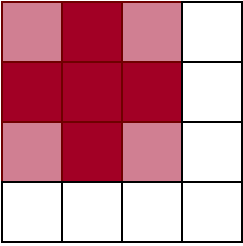
\includegraphics[width=\textwidth]{assets/r1.pdf}
        \caption{Кадр №1}
    \end{subfigure}
    \begin{subfigure}{0.17\textwidth}
        \centering
        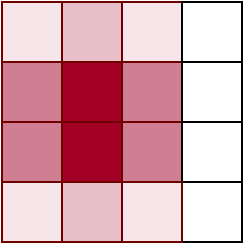
\includegraphics[width=\textwidth]{assets/r2.pdf}
        \caption{Кадр №2}
    \end{subfigure}
    \begin{subfigure}{0.17\textwidth}
        \centering
        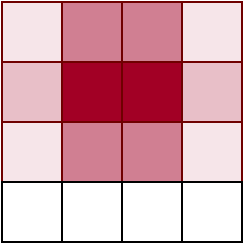
\includegraphics[width=\textwidth]{assets/r3.pdf}
        \caption{Кадр №3}
    \end{subfigure}
    \begin{subfigure}{0.17\textwidth}
        \centering
        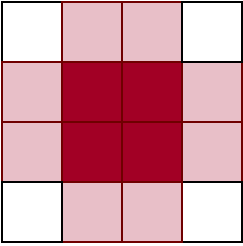
\includegraphics[width=\textwidth]{assets/r4.pdf}
        \caption{Кадр №4}
    \end{subfigure}
    \caption{Пример набора кадров одного и того же объекта, регистрируемого фотосистемой}
    \label{circles}
\end{figure}

На рисунке \ref{big} представлена связь между пикселями НР изображения и пикселями ВР изображения.

\begin{figure}[H]
	\centering
	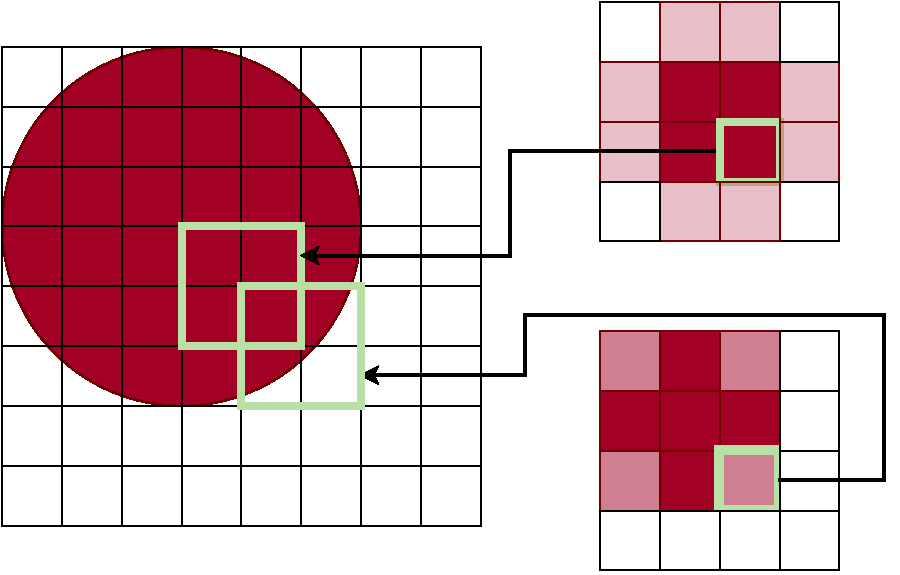
\includegraphics[scale=0.4]{assets/big}
	\caption{Связь между пикселями НР изображения и пикселями ВР изображения}
	\label{big}
\end{figure}

Как можно заметить, источником дополнительной информации для решения поставленной задачи являются субпиксельные сдвиги между кадрами набора.

Представим желаемое изображение ВР размером $N = L_1 N_1 \times L_2 N_2$ как вектор $x = [x_1, x_2, ..., x_N]^T$. Параметры $L_1$ и $L_2$ представляют собой коэффициенты понижения дискретизации в наблюдении для горизонтального и вертикального направлений соответственно. 

Таким образом, каждое изображение НР имеет размерность $M = N_1 \times N_2$. Аналогично представим каждое изображение НР в виде вектора $y_k~=~[y_{k_1}, y_{k_2}, ..., y_{k_M}]^T$, где $k = \overline{1, p}$, $p$ --- размер входного набора.

Для получения изображения высокого разрешения $x$ методом суперразрешения рассматривается следующая система уравнений~\cite{model}:

\begin{equation}
    A_kx = y_k,
\end{equation}

где оператор $A_kx$ в общем случае представляется в виде выражения~(\ref{fig:akx}).

\begin{equation}\label{fig:akx}
    A_kx = D\cdot B_k\cdot M_k \cdot x + n_k,
\end{equation}

где:

\begin{itemize}
    \item D --- матрица движения фотосистемы (сдвиг, поворот и т.д.);
    \item $B_k$ --- матрица размытия (может быть вызвано оптической системой, относительным движением между фотосистемой и сценой, а также функцией рассеяния в датчике фотосистемы);
    \item $M_k$ --- матрица понижения размерности (генерирует изображение НР путем наложения, т.е. алиасинга). %Важно учитывать, что при реконструкции по нескольким кадрам размерность этой матрицы может варьироваться;
    \item $n_k$ --- вектор шума.
\end{itemize}

Возможна более короткая форма записи:

\begin{equation}
    A_kx = W_k\cdot x + n_k = y_k,
\end{equation}

где матрица $W_k$ размером $(N_1, N_2)^2 \times L_1 N_1 L_2 N_2$ представляет собой вклад пикселей изображения $x$ в изображение $y_k$ посредством размытия, движения и субдискретизации.

\clearpage

\section{Частотные методы}

Данная группа методов суперрезолюции ориентирована на увеличение разрешения изображения посредством анализа частотных характеристик кадров. Классическим математическим аппаратом для подобных задач является Фурье~--~анализ.

Этот подход основывается на следующих принципах:

\begin{enumerate}
    \item Свойство сдвига преобразования Фурье: $f(\widehat{x - x_0}) = e^{-i\omega x_0}\hat{f}(\omega)$.
    \item Взаимосвязь между непрерывным преобразованием Фурье исходного изображения ВР и дискретным преобразованием Фурье наблюдаемых изображений НР.
    \item Частотный диапазон изображения ограничен.
\end{enumerate}

Пусть $x(t_1, t_2)$ --- непрерывное изображение ВР, $X(w_1, w_2)$ --- соответствующее ему непрерывное преобразование Фурье, $y_k[n_1, n_2]$ --- $k$~--~ое изображение НР, $Y(\Omega_1, \Omega_2)$ --- соответствующее ему дискретное преобразование Фурье.

Глобальные сдвиги, которые являются единственным движением, рассматриваемым в подходе частотной группы методов, порождают следующее уравнение для изображений НР:

\begin{equation}
    x_k(t_1, t_2) = x(t_1 + \delta_{k_1}, t_2 + \delta_{k_2}),
\end{equation}

где $\delta_{k_1}$ и $\delta_{k_2}$ --- величины субпиксельных сдвигов между кадрами.

Согласно свойству сдвига преобразования Фурье:

\begin{equation}
    X_k(w_1, w_2) = exp[i\cdot2\pi(\delta_{k_1}\cdot w_1 + \delta_{k_2}\cdot w_2)]\cdot X(w_1, w_2).
\end{equation}

Смещенное изображение $x_k(t_1, t_2)$ дискретизируется с периодами $T_1$ и $T_2$ для создания наблюдаемого изображения НР $y_k[n_1, n_2]$~\cite{frequency}.

Таким образом, взаимосвязь между $X(w_1, w_2)$ и $Y(\Omega_1, \Omega_2)$ может быть описана в виде (\ref{eqv:link}).

\begin{equation}\label{eqv:link}
    Y(\Omega_1, \Omega_2) = \cfrac{1}{T_1\cdot T_2} \cdot \sum_{n_1 = 0}^{L_1 - 1} \sum_{n_2 = 0}^{L_2 - 1} X_k \cdot \left[\cfrac{2\pi}{T_1} \cdot \left(\cfrac{\Omega_1}{N_1} + n_1\right), \cfrac{2\pi}{T_2} \cdot \left(\cfrac{\Omega_2}{N_2} + n_2\right)\right].
\end{equation}

Учитывая, что функция $X$ финитна, матрично~--~векторная форма уравнения может быть записана в виде (\ref{eqv:yfx}).

\begin{equation}\label{eqv:yfx}
    Y = \Phi X.
\end{equation}

\section{Пространственные методы}

\subsection{Регистрация~--~интерполяция~--~восстановление}

Линейный подход к решению задачи суперразрешения на основе интерполяции является наиболее тривиальным, однако в связи с этим имеет ряд существенных недостатков: возникновение алиасинга (эффект <<лесенки>>), размытия и эффекта Гиббса (проявляется в виде ореолов возле резких перепадов интенсивности). 

Выделяют следующие этапы метода:

\begin{enumerate}
    \item Непосредственно регистрация изображений НР и их последующее выравнивание до субпиксельной точности. 
    \item Интерполяция полученных изображений НР (например, с использованием метода ближайших соседей, интерполяции Ланцоша, линейной, биполярной, бикубической или гауссовской интерполяции).
    \item Устранение размытия и помех (решение инверсной задачи) --- получение изображения ВР.
\end{enumerate}

На рисунке \ref{fig:interpolation} представлен алгоритм суперрезолюции на основе рассматриваемого подхода~\cite{p}.

\begin{figure}[H]
	\centering
	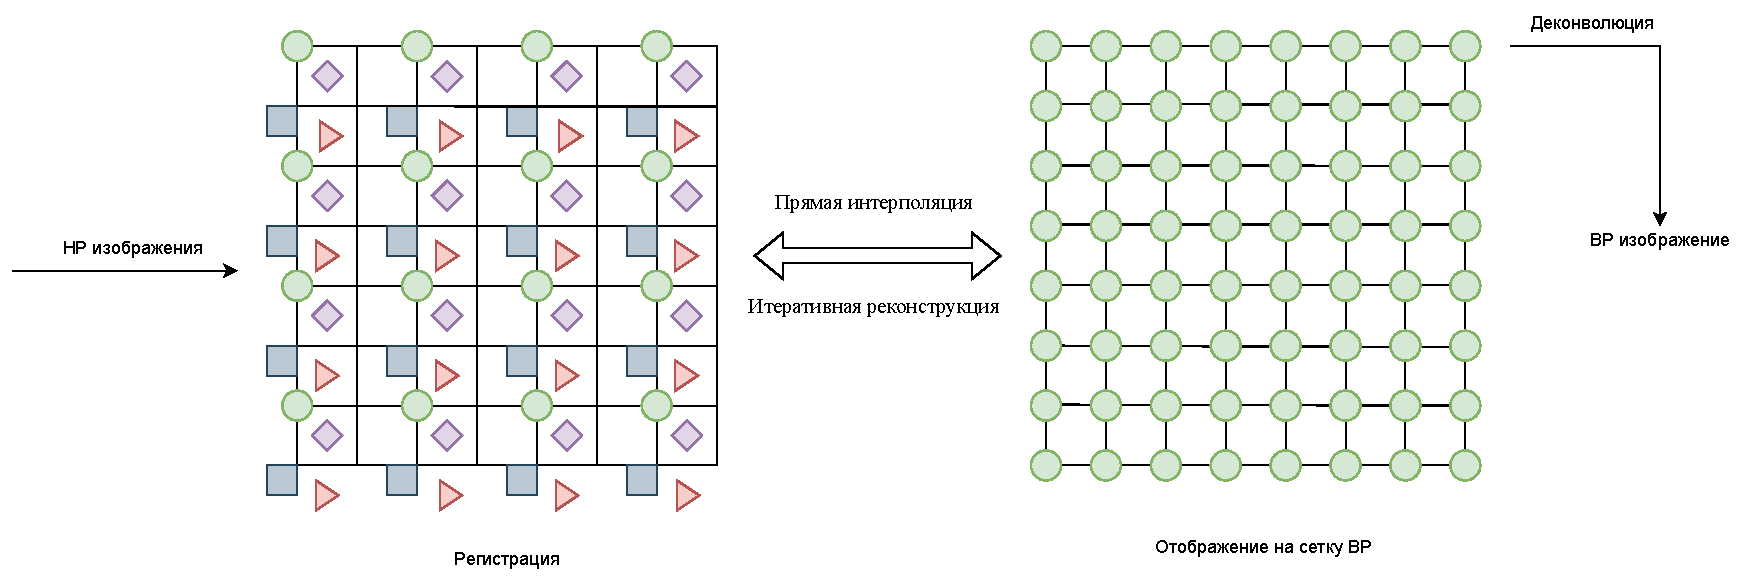
\includegraphics[scale=0.55]{assets/inerpolation.pdf}
	\caption{Алгоритм суперрезолюции на основе подхода регистрация~--~интерполяция~--~восстановление}
	\label{fig:interpolation}
\end{figure}

Изображение представляется в виде функции, пиксели изображения --- точки, в которых значение функции известно. Суть метода заключается в вычислении значения функции в промежуточных точках.

\subsection{Примеро~--~ориентированные методы}

Данная группа методов реализовывает подход, основанный на глубоком обучении~\cite{patch}. Создается набор изображений (изображения ВР подвергают деградации (см. рисунок \ref{model}) и формируется пара (ВР;НР)), который затем используется для анализа деталей, соответствующих отдельным областям цифрового изображения. Выявленные взаимосвязи используются для прогнозирования мелких деталей на других изображениях.

Рассмотрим алгоритм, предложенный в работе <<Example~--~Based Super~--~Resolution>>~\cite{example}. На рисунке \ref{tiger} представлены изображения, иллюстрирующие суть алгоритма.

\begin{figure}[!h]
    \centering
    \begin{subfigure}{0.25\textwidth}
        \centering
        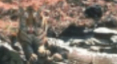
\includegraphics[width=\textwidth]{assets/tiger_a}
        \caption{}
    \end{subfigure}
    \begin{subfigure}{0.35\textwidth}
        \centering
        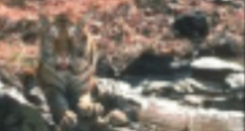
\includegraphics[width=\textwidth]{assets/tiger_b}
        \caption{}
    \end{subfigure}
    \begin{subfigure}{0.35\textwidth}
        \centering
        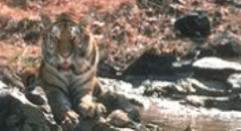
\includegraphics[width=\textwidth]{assets/tiger_c}
        \caption{}
    \end{subfigure}
    \begin{subfigure}{0.33\textwidth}
        \centering
        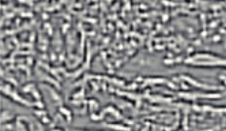
\includegraphics[width=\textwidth]{assets/tiger_d}
        \caption{}
    \end{subfigure}
    \vspace{1cm}
    \begin{subfigure}{0.35\textwidth}
        \centering
        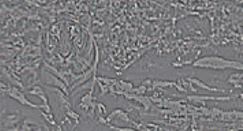
\includegraphics[width=\textwidth]{assets/tiger_e}
        \caption{}
    \end{subfigure}
    \caption{Изображения, иллюстрирующие этапы алгоритма}
    \label{tiger}
\end{figure}

На вход алгоритму подается исходное изображение НР \ref{tiger}.a и соответствующее ему изображение ВР \ref{tiger}.c. Изображение \ref{tiger}.b --- результат интерполяции исходного изображения. Эта операция позволяет получить изображение нужного размера, но изображение по~--~прежнему не содержит достаточно сведений о деталях.

\clearpage

Следующий шаг --- сохранить в базу данных каждый патч изображения ВР, соответствующий каждому патчу изображения НР (под патчем понимается небольшой участок изображения, обычно размером $5\times5$ или $7 \times 7$). 

В виду того, что данная операция требует существенного количества памяти, изображения НР предварительно обрабатываются, чтобы устранить вариативность и сделать обучающие наборы максимально применимыми.

Предполагается, что высокочастотные компоненты патчей наиболее важны для предсказаний. В связи с этим к изображению \ref{tiger}.b применяется фильтр низких частот. 

Также предполагается, что взаимосвязь между участками изображений с высоким и низким разрешением по существу не зависит от локального контраста изображения, в связи с чем применяется операция нормализации контраста.

На рисунке \ref{fig:patch_1} представлен пример базы данных патчей согласно описанному выше методу.

\begin{figure}[H]
	\centering
	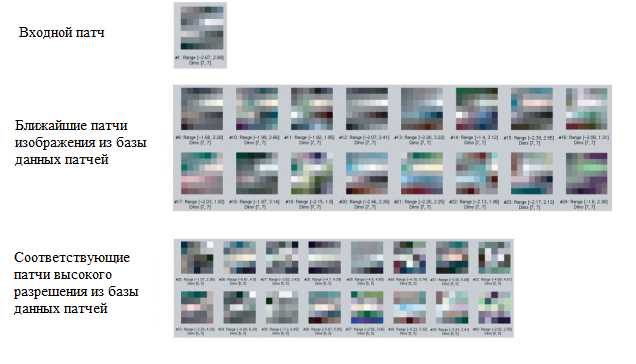
\includegraphics[scale=1.05]{assets/patch_2.png}
	\caption{Пример базы данных патчей}
	\label{fig:patch_1}
\end{figure}

\clearpage

Таким образом, изображения \ref{tiger}.d и \ref{tiger}.e соответствуют изображениям \ref{tiger}.b  и \ref{tiger}.c, подвергнутых описанным операциям. Полученная пара изображений используется для обучения.

Алгоритм суперрезолюции осуществляется путем разбиения кадра на патчи и составления изображения ВР путем перебора соответствующих патчей в базе данных. На рисунке \ref{fig:patch_2} представлен пример сравнения патчей.

\begin{figure}[H]
	\centering
	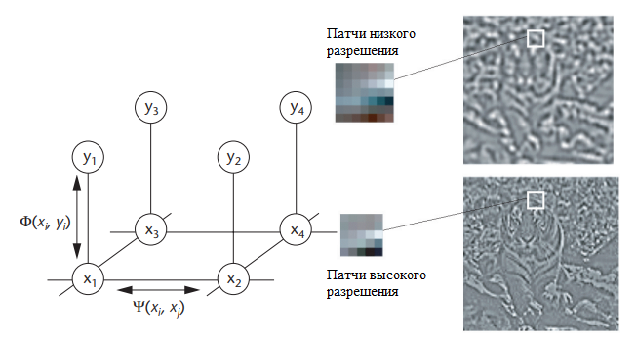
\includegraphics[scale=1.0]{assets/patch_1.png}
	\caption{Пример сравнения патчей}
	\label{fig:patch_2}
\end{figure}

\subsection{Реконструкция с регуляризацией}

Задача реконструкции (решение обратной задачи) изображения ВР является некорректной в виду недостаточного количества информации о деталях и отсутствия априорной информации о функции размытия в общем случае. Методы регуляризации сводят некорректно поставленную задачу к корректной посредством введения дополнительных ограничений. 

В данном разделе представлены детерминированные и стохастические (статистические) методы реконструкции.

\clearpage

\subsubsection{Детерминированные регуляризационные методы}

Оценив параметры регистрации, можно полностью уточнить модель наблюдения (1.2). Рассматриваемый подход решает обратную задачу, используя априорную информацию о решении, которая может быть использована для корректной постановки задачи.

Рассмотрим формулировку метода наименьших квадратов~\cite{mnk}, выбрав $x$ для минимизации Лангранжиана:

\begin{equation}
    \sum_{k=1}^{p} ||y_k - W_k||^2 + \alpha ||Cx||^2,
\end{equation}

где оператор $C$ --- фильтр верхних частот, $||\cdot||$ --- $l_2$ -- норма, $\alpha$ --- параметр регуляризации (множитель Лангранжа), контролирующий компромисс между точностью данных. Чем больше значение $\alpha$, тем более гладкое решение. Это может быть полезным, когда доступно небольшое количество изображений НР, а также когда точность информации на изображении низкая в виду зашумленности и ошибок регистрации, однако когда количество зображений НР достаточно большое и уровень шума в пределах нормы, то меньше значения $\alpha$ могут дать лучший результат.

Основные методы детерминированной итеративной регуляризации решают следующую задачу:

\begin{equation}
    \left[\sum_{k=1}^{p} W_k^TW_k + \alpha C^TC\right]\hat{x} = \sum_{k=1}^{p} W_k^Ty_k, 
\end{equation}

что приводит к формулировке следующей рекуррентной формулы для~$\hat{x}$:

\begin{equation}
    \hat{x}^{n+1} = \hat{x}^n + \beta \left[\sum_{k=1}^{p} W_k^T (y_k - W_k \hat{x}^n) - \alpha C^TC \hat{x}^n \right],
\end{equation}

где $\beta$ --- параметр сходимости.

 \subsubsection{Стохастические регуляризационные методы}

Данная группа методов основана на байесовской статистике и используется, когда можно установить апостериорную функцию плотности исходного изображения.

Оценка $x$ с помощью метода максимального правдоподобия максимизирует апостериорную функцию плотности $P(x|y_k)$ относительно $x$:

\begin{equation}
    x = \arg \max P(x | y_1, y_2, ..., y_p).
\end{equation}

Запишем задачу максимизации, применив логарифмирование, а также теорему Байеса к условной вероятности:

\begin{equation}
    x = \arg \max \{ln P(y_1, y_2, ..., y_p | x) + ln P(x)\}.
\end{equation}

Здесь и априорная модель изображения $P(x)$, и условная плотность $P(y_1, y_2, ..., y_p | x)$ будут определяться априорной информацией об изображении ВР и статической информацией о шуме. Поскольку этот метод учитывает априорные ограничения, то предоставляется стабильная оценка изображения ВР.

Байесовская оценка также может быть осуществлена с использованием маркова случайного поля, описываемого приором Гиббса:

\begin{equation}
    \displaystyle P(X = x) = \cfrac{1}{Z} exp\{-U(x)\} = \cfrac{1}{Z} exp\{-\sum_{i\in S}^{}\phi_i(x)\}, 
\end{equation}

где $Z$ --- константа нормализации, $U(x)$ --- энергетическая функция, $\phi_i(x)$ --- функция производной изображения, которая зависит от значения пикселей, расположенных внутри $S$.

Главным преимуществом байесовской модели является использование предварительной модели изображения с сохранением краев изображения. В таком случае задача формулируется следующим образом~\cite{map}:

\begin{equation}
    x = \arg \min [\sum_{k=1}^{p}||y - W_k\cdot x]||^2 + \alpha \sum_{}^{}\phi(x)].
\end{equation}

\subsection{Методы резолюции на основе теории множеств}

Данная группа методов POCS (англ. \textit{Projection Onto Convex Sets})~\cite{pocs, pocs2} осуществляет альтернативный итеративный подход к учету априорных знаний для решения задачи реконструкции.

Согласно методу POCS, учет априорных знаний в решение можно интерпретировать как наложение ограничения на то, чтобы решение было членом замкнутого выпуклого множества $C_i$, которое определяется как набор векторов, удовлетворяющих определенному свойству. Ограничение представляет собой предположительные сведения о гладкости, структуре, текстуре и других характеристиках изображения.

Если множества ограничений имеют непустое пересечение, то решение, принадлежащее множеству пересечений $C_s = \cap _{i=1}^{m}C_i$ (которое тоже является выпуклым множеством), можно найти, чередуя проекции на эти выпуклые множества.

После каждой итерации проекции обновляется текущее приближение к высокоразрешенному изображению. Этот процесс повторяется до тех пор, пока не достигнута сходимость или другие критерии остановки.    

На рисунке \ref{fig:convex} представлена иллюстрация метода суперрезолюции на основе теории множеств.

\begin{figure}[H]
	\centering
	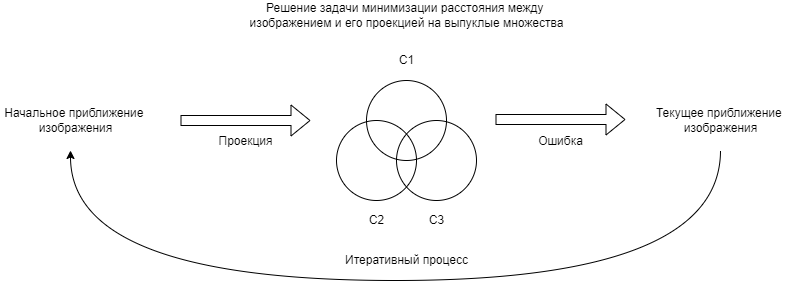
\includegraphics[scale=0.6]{assets/convex.png}
	\caption{Метод суперрезолюции на основе теории множеств}
	\label{fig:convex}
\end{figure}

\section{Методы на основе нейронных сетей}

Сверточные нейронные сети в области распознавания образов на изображениях и их классификации нашли широкое применение, что объясняется достаточно высоким качеством решения подобных задач.

Архитектура сети получила название в виду использования операции свертки. На рисунке \ref{conv} представлен пример выполнения операции. Для вычисления новых значений используется т.н. ядро свертки. На представленном примере ядром является матрица серого цвета размером $3\times3$ ячейки.

\begin{figure}[H]
	\centering
	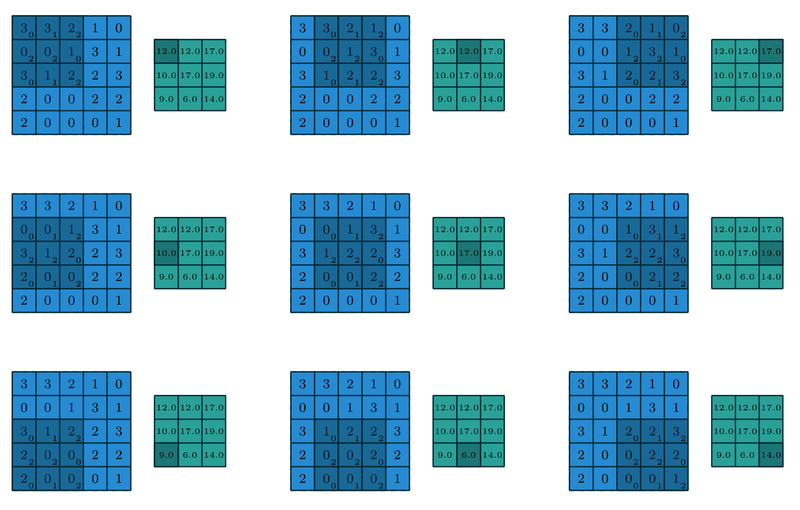
\includegraphics[scale=1.25]{assets/convolution_example}
	\caption{Пример свертки цифрового изображения}
	\label{conv}
\end{figure}

На рисунке \ref{cnn} представлена типовая архитектура сверточной нейронной сети.

\begin{figure}[!h]
	\centering
	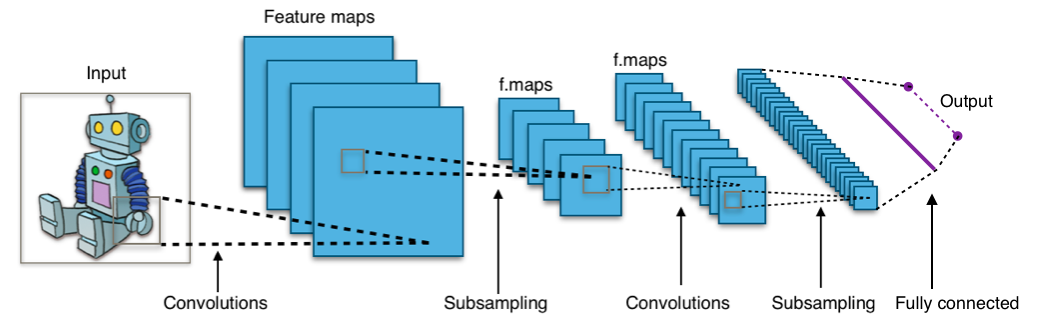
\includegraphics[scale=0.35]{assets/typical_cnn.png}
	\caption{Типовая архитектура сверточной нейронной сети}
	\label{cnn}
\end{figure}

Как можно увидеть, СНС состоит из 3 типов слоев \cite{cnn, cnn2, cnn3}:

\begin{enumerate}
    \item Слой свертки --- основной блок СНС, производящий свертку входной матрицы с ядром свертки. Количество ядер равно количеству карт признаков, выделяемых на изображении.
    \item Слой пуллинга, или субдескритизация --- данный слой принимает результат свертки предыдущего слоя в вид матрицы и сжимает данную матрицу с целью выделения низкоуровненвых признаков.
    \item Полносвязный слой --- на данный слой подается одномерный вектор от стоящего перед ним слоя, причем данный вектор получен из матрицы путем записи ее элементов построчно в одну строку.
\end{enumerate}

\subsection{Оптимизация глубоких нейронных сетей}

Одна из ключевых задач в тренировке глубоких нейронных сетей --- оптимизация их параметров. Вследствие большого совокупного числа параметров на всех слоях нейронной сети применение методов второго порядка (таких как BFGS, SR1 и других квазиньютоновских методов) крайне затруднительно, а методы нулевого порядка в большинстве случаев не позволяют найти качественное решение за приемлемое время.

По этой причине для оптимизации глубоких и в том числе сверточных нейронных сетей, наиболее распространены методы первого порядка, требующие лишь знания градиента сети как функции от ее параметров. Сперва в качестве параметров алгоритма оптимизации глубоких нейронных сетей использовался градиентный спуск. Впоследствии было продемонстрировано, что градиентный спуск хоть и не требователен к вычислительным ресурсам, но значительно уступает многим методам первого порядка в скорости сходимости.

\subsection{Проекция~--~аппроксимация~--~восстановление}

Исходя из приведенных выше соображений, были разработаны методы, основанные на подходе проекции-аппроксимации-восстановления~\cite{pav, senov}. 

Под подходом проекции–аппроксимации–восстановления понимается следующая процедура (далее обозначаемая акронимом
ПАВ):

\begin{enumerate}
    \item Проекция: проекция нескольких последних точек из оригинального пространства в пространство меньшей размерности посредством умножения на специальным образом построенную прямоугольную матрицу с ортонормальными строками.
    \item Аппроксимация:построение квадратичного полинома, аппроксимирующего полученные проекции точек и соответствующие им значения целевой функции. 
    \item Восстановление: аппроксимация параметров целевой функции (например, Гессиана, точки минимума) в оригинальном пространстве на основе полученного полинома в пространстве меньшей размерности и прямоугольной матрицы из первого пункта.
\end{enumerate}